 \chapter{Analisis dan Perancangan}


\section{Analisis}

Pada kondisi saat ini, alokasi petugas pengumpulan data di BPS dilakukan pada saat perancangan. Sebelum proses pengumpulan data dilakukan, dan lokasi pencacahan telah diketahui (berdasarkan metode sampling yang digunakan), petugas kemudian direkrut dan dialokasikan kepada lokasi pencacahan terdekat. Pengalokasian lokasi pencacahan terhadap masing-masing pencacah, seringkali dilakukan secara subyektif, sehingga menyebabkan variasi waktu penyelesaian tinggi. 


Metode MTSP dan berbagai variasinya dapat digunakan untuk mengatasi pengalokasian diatas. Variasi MTSP yang dapat digunakan dalam permasalahan ini antara lain: 1) Menggunakan lebih dari satu pencacah, dimana masing-masing pencacah memulai dari \textit{depot} yang berbeda-beda; 2) Penimbang dari setiap lokasi pencacahan dengan lokasi lainnya direpresentasikan dengan waktu tempuh. Waktu tempuh lebih representatif untuk digunakan sebagai penimbang dibanding jarak, karena jarak tidak memperhitungkan kesulitan akses. 


Untuk menggambarkan bagaimana MTSP dapat digunakan untuk mengatasi masalah ini, maka perlu dilakukan eksperimen. Eksperimen dilakukan dengan langkah-langkah seperti berikut :


\subsection{Dataset}

\subsubsection{Lokasi Pencacahan}

Lokasi pencacahan yang digunakan merupakan data \textit{real} (bukan dummy), yang merupakan lokasi nagari/kelurahan di Kab. Pesisir Selatan, Provinsi Sumatera Barat. Data lokasi pencacahan yang digunakan dalam eksperimen ini sebanyak 182 lokasi. Contoh data lokasi pencacahan dapat dilihat pada Tabel. \ref{tbl:enumeration_locations}, sementara data lokasi pencacahan secara lengkap dapat dilihat pada Tabel. \ref{tbl:enumeration_locations_full}.


\begin{table*}\centering
\ra{1.3}
\caption{Lokasi Pencacahan}
\label{tbl:enumeration_locations}
\begin{tabular}{lcc}
\toprule
& \multicolumn{2}{c}{Koordinat}\\
\cmidrule{2-3}
& Latitude & Longitude\\ 
\midrule
1302011001 & -2.3504 & 101.1434\\ 
1302011002 & -2.4233 & 101.0285\\ 
1302011003 & -2.3798 & 101.0427\\ 
1302011004 & -2.3884 & 101.049\\ 
1302011005 & -2.3936 & 101.0546\\
...\\
1302110019 & -1.2387 & 100.4853\\ 
1302110020 & -1.1408 & 100.4938\\ 
1302110021 & -1.0883 & 100.4652\\ 
1302110022 & -1.0886 & 100.489\\ 
1302110023 & -1.1523 & 100.4978\\
\bottomrule
\end{tabular}
\end{table*}


\subsubsection{Pencacah}

Pada konsep MTSP, pencacah berperan sebagai \textit{salesman} yang harus berpindah dari satu lokasi ke lokasi lain secara berurutan. Pencacah juga diidentifikasi dengan \textit{depot}, yaitu lokasi dimana pencacah harus memulai dan mengakhiri. Dalam eksperimen ini digunakan 15 pencacah dengan lokasi \textit{depot} yang bervariasi. Tabel \ref{tbl:enumerator} adalah contoh data pencacah beserta lokasi \textit{depot}-nya yang digunakan dalam eksperimen ini, sementara data lengkap dapat dilihat pada Tabel \ref{tbl:enumerator_full}.


\begin{table*}\centering
\ra{1.3}
\caption{Pencacah}
\label{tbl:enumerator}
\begin{tabular}{lcc}
\toprule
& \multicolumn{2}{c}{Koordinat Depot}\\
\cmidrule{2-3}
& Latitude & Longitude\\ 
\midrule
1302011008 & -2.3905 & 101.1214\\
1302012003 & -2.199 & 101.1188\\
1302020006 & -2.1225 & 101.0687\\
...\\
1302100002 & -1.23265 & 100.54314\\
1302101005 & -1.19831 & 100.58078\\
1302110003 & -1.2475 & 100.4745\\
\bottomrule
\end{tabular}
\end{table*}


\subsubsection{Jarak dan Waktu Tempuh}

Jarak dan waktu tempuh antar node digunakan sebagai penimbang dalam penentuan rekomendasi lokasi. Penghitungan jarak dan waktu tempuh, selain dapat dilakukan secara manual (berdasarkan hasil survei atau perkiraan \textit{subject matter}), dapat juga didekati dengan menggunakan Google Directions API \citep{google_google_2016}. Keuntungan dengan menggunakan Google Direction API adalah jarak dan waktu yang dihitung telah memperhitungkan rute tercepat, kondisi geografis, kemacetan lalu-lintas, dan moda yang digunakan. Adapun kekurangan dari Google Direction API adalah jumlah \textit{requests} yang dapat dikirimkah sangat terbatas, hanya 1.000 \textit{requests} per hari per akun, sementara jumlah waktu dan jarak yang harus dihitung sejumlah $ nx(n-1)/2 = 182x187/2 = 16.471 $. Listing \ref{lst:google_direction_api_request} memuat contoh \textit{requests} dengan Google Direction API, dan Gambar \ref{fig:google_direction_api_response} adalah contoh responnya.


\begin{listing}
    \caption{Google Direction API Request}
    \label{lst:google_direction_api_request}
%    \begin{minted}[showspaces=false, breaklines=true, escapeinside=||]{http}
%https://maps.googleapis.com/maps/api/directions/json?origin=originx,originy&destination=destx,desty&departure_time=timestamp&traffic_model=best_guess&key=APIKEY
%	\end{minted}
\end{listing}


\begin{figure}[h]
    \centering
    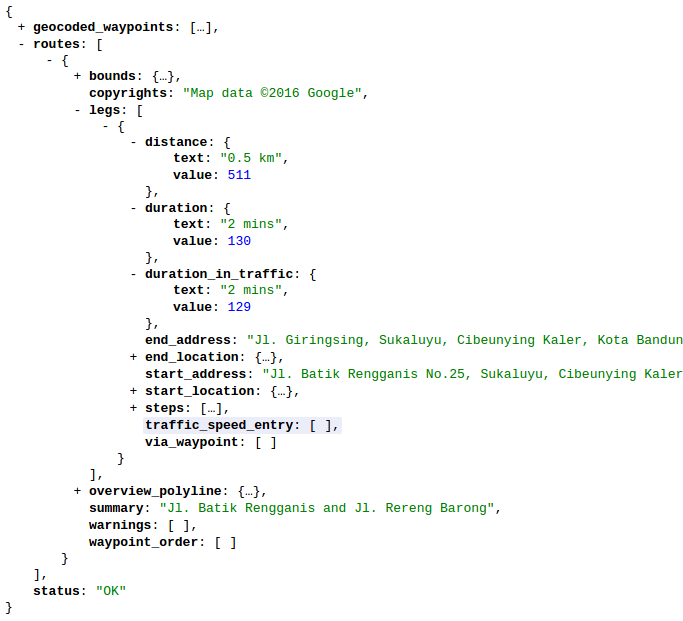
\includegraphics[width=\textwidth]{../../Resources/Images/google_direction_api_response}
    \caption{Google Direction API Response}
    \label{fig:google_direction_api_response}
\end{figure}


Contoh matrix jarak dan waktu tempuh dapat dilihat pada Tabel. \ref{tbl:distance_duration_matrix}, sementara data secara lengkap dapat dilihat pada Tabel. \ref{tbl:distance_duration_matrix_full}. Sebagai catatan, jika lokasi \textit{depot} dari pencacah bukan salah satu dari lokasi pencacahan, maka lokasi \textit{depot} juga harus disertakan dalam matriks jarak dan waktu tempuh.


\begin{table*}\centering
\ra{1.3}
\caption{Matriks Jarak dan Waktu Tempuh}
\label{tbl:distance_duration_matrix}
\begin{tabular}{llcc}
\toprule
Lokasi A & Lokasi B & Jarak & Waktu Tempuh\\
\midrule
1302021001 & 1302021003 & 11119 & 1055\\
1302021001 & 1302021002 & 9373 & 868\\
1302021001 & 1302021005 & 490 & 38\\
1302021001 & 1302021004 & 22760 & 2044\\
1302021001 & 1302021007 & 10228 & 950\\
...\\
1302040015 & 1302100015 & 99719 & 9682\\
1302040015 & 1302012010 & 77889 & 8305\\
1302040014 & 1302100015 & 103893 & 9984\\
1302040014 & 1302012010 & 73561 & 7546\\
1302100015 & 1302012010 & 171636 & 16801\\
\bottomrule
\end{tabular}
\end{table*}


\subsection{\textit{Library} dan Implementasi}

Pada eksperimen ini digunakan jsprit \citep{jsprit_jsprit_2014}, sebuah library berbasis java yang dapat digunakan untuk menyelesaikan permasalahan traveling salesman (TSP) dan vehicle routing problems (VRP). Jsprit mencakup berbagai skenario, antara lain : \textit{pickups and deliveries}, \textit{back hauls}, \textit{heterogeneous fleets}, \textit{finite and infinite fleets}, \textit{multiple depots}, \textit{time windows}, \textit{open routes}, \textit{different start and end locations}, \textit{multiple capacity dimensions}, \textit{initial loads}, \textit{skills}, dll. Cara kerja jsprit sangat terstruktur, mulai dari pendefinisan masalah, pemilihan algoritma, pencarian solusi, dan terakhir pemilihan solusi terbaik.


\subsubsection{Definisi Masalah}

\begin{listing}
    \caption{Definisi Pencacah dari File}
    \label{lst:jsprit_define_enumerators}
	\inputminted[showspaces=false, breaklines=true]{java}{../../Resources/Snippets/jsprit_enumerator.java}    
    
%    \begin{minted}[showspaces=false,breaklines=true]{java}
%VehicleTypeImpl.Builder vehicleTypeBuilder = VehicleTypeImpl.Builder.newInstance("enumerator");
%vehicleTypeBuilder.setCostPerDistance(0);
%vehicleTypeBuilder.setCostPerTransportTime(1);
%vehicleTypeBuilder.setCostPerServiceTime(1);
%VehicleType vehicleType = vehicleTypeBuilder.build();
%
%try {
%    CSVReader reader = new CSVReader(new FileReader(csvEnum));
%    reader.readNext();
%
%    String [] line;
%    while ((line = reader.readNext()) != null) {
%        VehicleImpl.Builder builder = VehicleImpl.Builder.newInstance(line[0]);
%
%        try {
%            Location loc = Location.Builder.newInstance()
%                    .setId(line[0])
%                    .setCoordinate(Coordinate.newInstance(Double.parseDouble(line[2]),
%                            Double.parseDouble(line[1])))
%                    .build();
%            builder.setStartLocation(loc);
%        } catch (Exception e) {}
%
%
%        builder.setType(vehicleType);
%        VehicleImpl vehicle = builder.build();
%        vrpBuilder.addVehicle(vehicle);
%    }
%
%} catch (FileNotFoundException e) {
%    e.printStackTrace();
%} catch (IOException e) {
%    e.printStackTrace();
%}
%	\end{minted}
\end{listing}


\section{Garis Besar Perancangan}

Alur kerja perancangan dimulai dengan dengan mengidentifikasi blok sensus yang akan dilakukan pendataan padanya, serta menentukan jumlah pencacah yang akan digunakan. Kedua permasalahan ini tidak akan dibahas terlalu mendalam dalam penelitian ini. Lokasi pencacahan telah ditentukan dalam fase perancangan sensus dan survei, mengikuti sebuah metodologi tertentu. Sementara jumlah pencacahan juga telah ditentukan, mengikuti jumlah sampel dan berbagai persyaratan tertentu, seperti waktu dan biaya.


Selanjutnya, setiap pencacah akan dialokasikan kepada blok sensus yang akan dicacah dengan menggunakan metode MTSP, sebagaimana diformulasikan oleh \citep{bektas_multiple_2006}, dengan ketentuan setiap pencacah dapat memulai dan mengakhiri pada \textit{depot} yang berbeda-beda. Setelah model diperoleh, setiap pencacah akan mengunjungi lokasi pertama dari rekomendasi. Setelah selesai kunjungan, lokasi akan disimpan dalam \textit{tabu list} dengan menggunakan metode pub-sub \citep{chen_efficient_2003}. Model baru akan digenerate setiap kali terdapat \textit{request} dari salah satu pencacah. Setiap kali model di-\textit{generate}, \textit{tabu search} \citep{glover_tabu_1989, glover_tabu_1990} yang memanfaatkan \textit{tabu list} akan digunakan untuk memastikan tidak terdapat \textit{conflict}. Setelah model baru selesai di-\textit{generate}, maka mudel akan di-\textit{publish} kepada setiap pencacah yang telah men-\textit{subscribe}.


\begin{figure}[h]
    \centering
    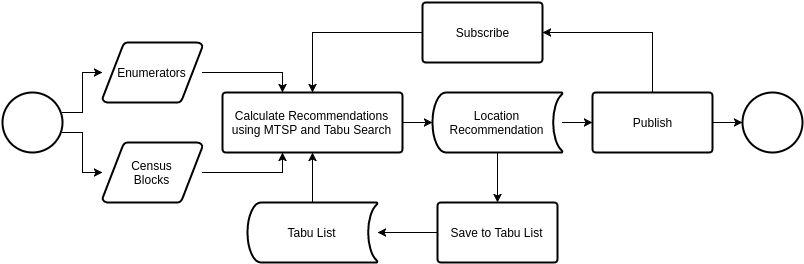
\includegraphics[width=\textwidth]{../../Resources/Images/design_overview}
    \caption{Garis Besar Sistem Usulan}
    \label{fig:design_overview}
\end{figure}


\section{Penyusunan Rekomendasi}

Pada tahap perumusan rekomendasi, input data yang terdiri dari data pencacah dan data blok sensus akan dioleh menjadi rekomendasi path yang harus dikunjungi. Proses penyusunan rekomendasi menggunakan metode \textit{Multiple Travelling Salesman Problem} (MTSP), yang merupakan pengembangan dari metode klasik \textit{Travelling Salesman Problem} (TSP).


Metode MTSP yang digunakan dalam masalah ini memiliki beberapa \textit{requirements}, antara lain:

\begin{itemize}
\item Jumlah \textit{depot} \\
MTSP dapat menggunakan lebih dari satu depot, dengan $ m_{j} $ \textit{salesman} untuk setiap depot $ j $. Pada permasalahan ini menggunakan \textit{non-fixed destination}, sehingga pencacahan tidak perlu kembali ke lokasi dimana pencacahan dimulai.
\item Jumlah \textit{salesman} \\
Jumlah \textit{salesman} yang digunakan dapat berupa \textit{fixed number} $ m $, atau dinamis dengan dibatasi jumlah maksimal $ max(m) $. Pada permasalahan ini digunakan \textit{fixed number} $ m $ pencacah.
\item \textit{Fixed charges} \\
Jika jumlah \textit{salesman} dinamis, maka bisa juga masing-masing \textit{salesman} dibatasi dengan sejumlah biaya tertentu. Pada permasalahan ini tidak digunakan \textit{fixed charges}.
\item Waktu kunjungan (\textit{time windows}) \\
\textit{Time windows} merepresentasikan waktu yang dihabiskan selama kunjugan dalam sebuah \textit{node}. Pada kasus ini \textit{time windows} tidak dapat ditentukan karena tidak tersedianya informasi, sehingga dianggap tidak menggunakan \textit{time windows}.
\end{itemize}


Requirements di atas, secara global dapat disederhanakan dalam tabel-tebel berikut. Tabel \ref{tbl:enumerators_overview} menunjukkan rancangan pencacah beserta koordinat \textit{depot}-nya, sementara Tabel \ref{tbl:census_blocks} menunjukkan rancangan blok sensus beserta koordinat dan \textit{time windows}-nya. Dalam fakta lapangan, jarak antara satu blok sensus dengan blok sensus yang lain tidaklah setara. Bisa jadi secara koordinat memiliki jarak yang berdekatan, tetapi secara akses tidaklah mudah. Untuk itu diperlukan sebuah tabel tambahan, yaitu tabel \textit{cost-matrix}, sebagaimana Tabel \ref{tbl:cost_matrix}. \textit{Cost} yang dimaksud disini adalah segala metrik yang dapat digunakan sebagai penimbang (\textit{weight}), misalnya: biaya, jarak, atau waktu tempuh.


\begin{table}[]
\centering
\caption{Table Pencacah}
\label{tbl:enumerators_overview}
\begin{tabular}{@{}lcc@{}}
\toprule
\multirow{2}{*}{Pencacah} & \multicolumn{2}{l}{\textit{Depot Coordinate}} \\ \cmidrule(l){2-3} 
                          & X                 & Y                \\ \midrule
Pencacah 1                & 20.0              & 20.0             \\
Pencacah 2                & 20.0              & 20.0             \\
Pencacah 3                & 30.0              & 40.0             \\
Pencacah 4                & 30.0              & 40.0             \\
...                       &                   &                  \\
Pencacah m                & x                 & y                \\ \bottomrule
\end{tabular}
\end{table}


\begin{table}[]
\centering
\caption{Tabel Blok Sensus}
\label{tbl:census_blocks}
\begin{tabular}{@{}lccc@{}}
\toprule
\multirow{2}{*}{Blok Sensus} & \multicolumn{2}{c}{Koordinat Lokasi} & \multirow{2}{*}{Time Windows} \\ \cmidrule(lr){2-3}
                             & X                 & Y                &                               \\ \midrule
001B                         & 62.0              & 63.0             & 0                             \\
002B                         & 63.0              & 69.0             & 0                             \\
003B                         & 46.0              & 10.0             & 0                             \\
004B                         & 61.0              & 33.0             & 0                             \\
...                          &                   &                  &                               \\
n                            & x                 & y                & 0                             \\ \bottomrule
\end{tabular}
\end{table}


\begin{table}[]
\centering
\caption{Table \textit{Cost-Matrix}}
\label{tbl:cost_matrix}
\begin{tabular}{@{}|c|c|c|c|c|c|c|@{}}
\toprule
        & 001B & 002B & 003B & 004B & ... & BS ke-n \\ \midrule
001B    & -    & 5    & 2    & 2    &     & ...     \\ \midrule
002B    &      & -    & 4    & 2    &     & ...     \\ \midrule
003B    &      &      & -    & 7    &     & ...     \\ \midrule
004B    &      &      &      & -    &     & ...     \\ \midrule
...     &      &      &      &      & -   & ...     \\ \midrule
BS ke-n &      &      &      &      &     & -       \\ \bottomrule
\end{tabular}
\end{table}


Tabel \textit{cost-matrix}, selain dapat didefinisikan secara manual (berdasarkan hasil survei atau perkiraan \textit{subject matter}), dapat juga didekati dengan menggunakan Google Directions API \citep{google_google_2016}. \textit{Request} yang digunakan menggunakan standar REST API, sementara \textit{response} yang ditampilkan dalam format JSON. Listing \ref{lst:google_direction_api_request} menunjukkan contoh \textit{request}, dan Gambar \ref{fig:google_direction_api_response} menunjukkan contoh \textit{response} dari Google Direction API.








%Gambar \ref{fig:mtsp_solution_example} berikut menunjukkan hasil rekomendasi dengan MTSP.
%
%
%\begin{figure}[h]
%    \centering
%    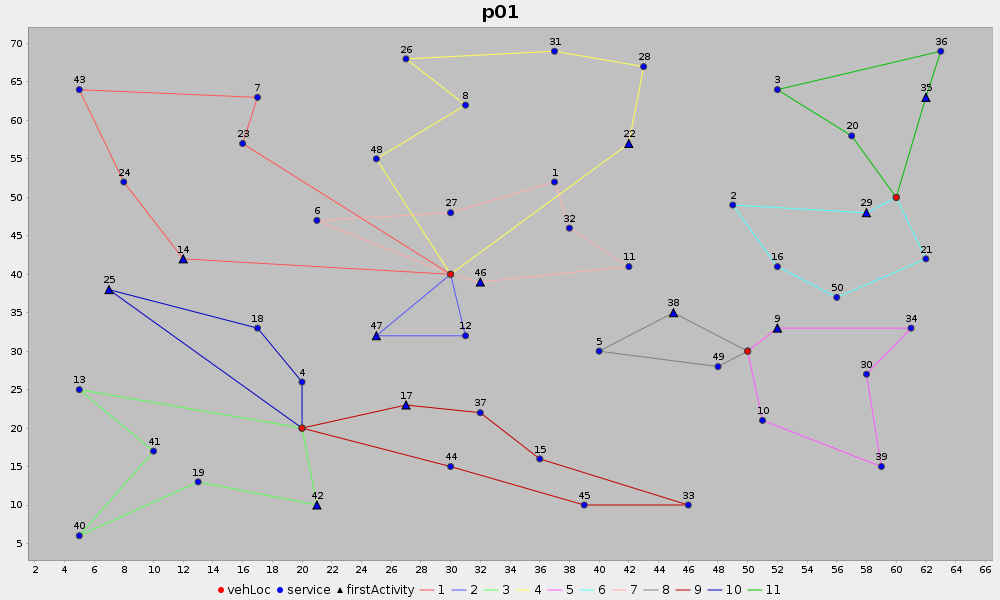
\includegraphics[width=\textwidth]{../../Resources/Images/mtsp_solution_example}
%    \caption{Contoh Hasil Rekomendasi}
%    \label{fig:mtsp_solution_example}
%\end{figure}


\section{Penyusunan \textit{Conflict Resolution}}


\section{\textit{Publish-Subscribe} Rekomendasi}
